\documentclass[twocolumn,aps,pra,floatfix,amsmath,amssymb,longbibliography]{revtex4-2}

\usepackage[T1]{fontenc}
\usepackage{amsthm}
\usepackage{booktabs}
\usepackage{xcolor}
\usepackage{tikz}
\usetikzlibrary{calc}
\usepackage[
  breaklinks=true,
  colorlinks=true,
  citecolor=blue,
  linkcolor=blue,
  urlcolor=blue
]{hyperref}
\usepackage{orcidlink}

\newtheorem{theorem}{Theorem}
\newtheorem{lemma}[theorem]{Lemma}
\newtheorem{proposition}[theorem]{Proposition}
\newtheorem{corollary}[theorem]{Corollary}
\theoremstyle{definition}
\newtheorem{definition}[theorem]{Definition}
\newtheorem{example}[theorem]{Example}
\theoremstyle{remark}
\newtheorem{remark}[theorem]{Remark}

\newcommand{\ii}{\mathrm{i}}
\newcommand{\C}{\mathbb C}
\newcommand{\R}{\mathbb R}
\newcommand{\Htwenty}{\mathsf H_{20}}
\newcommand{\Htwentyone}{\mathsf H_{21}}

% Context colors used in both octagon drawings.
\definecolor{ctx1}{RGB}{230,25,75}
\definecolor{ctx2}{RGB}{60,180,75}
\definecolor{ctx3}{RGB}{0,130,200}
\definecolor{ctx4}{RGB}{245,130,48}
\definecolor{ctx5}{RGB}{145,30,180}
\definecolor{ctx6}{RGB}{70,240,240}
\definecolor{ctx7}{RGB}{240,50,230}
\definecolor{ctx8}{RGB}{210,245,60}
\definecolor{ctx9}{RGB}{250,190,190}
\definecolor{ctx10}{RGB}{0,128,128}
\definecolor{ctx11}{RGB}{128,128,0}
\definecolor{ctx12}{RGB}{170,110,40}
\definecolor{ctx13}{RGB}{128,0,0}
\definecolor{ctx14}{RGB}{0,0,128}
\tikzset{ctxline/.style={line width=0.95pt,line cap=round}}

\newcommand{\twodotlabel}[5]{%
  \node[circle,fill=#1,draw=#1,minimum size=7.2pt,inner sep=0pt,
        label={[font=\scriptsize,label distance=0.7mm]#3:{#4}}] at #5 {};
  \node[circle,fill=#2,draw=#2,minimum size=4.2pt,inner sep=0pt] at #5 {};
}

\begin{document}

\title{Finite transition-probability witnesses separating real and complex qutrits}

\author{Mirko Navara\,\orcidlink{0000-0002-0880-5992}}
\affiliation{Faculty of Electrical Engineering, Czech Technical University in Prague,
Technick\'{a} 2, CZ-166~27 Prague 6, Czech Republic}
\email{navara@fel.cvut.cz}

\author{Karl Svozil\,\orcidlink{0000-0001-6554-2802}}
\affiliation{Institute for Theoretical Physics, TU Wien,
Wiedner Hauptstra{\ss}e 8-10/136, A-1040 Vienna, Austria}
\email{karl.svozil@tuwien.ac.at}

\date{\today}

\begin{abstract}
We construct two finite, dimension-bounded witnesses that separate complex
from real qutrit geometry in a calibrated prepare-and-projective-test
scenario.  Twenty and twenty-one labeled rays are used both as pure-state
preparations and as rank-one tests, so their transition probabilities are
squared ray overlaps.  The zero patterns form faithful orthogonality
hypergraphs with, respectively, 12 and 14 complete qutrit contexts.  Complex
qutrits reproduce both tables exactly; no calibrated reciprocal real-qutrit
model made of pure states and rank-one tests does.  The 20-ray obstruction is
the real rigidity of two rank-one decompositions of one positive operator.  The
21-ray obstruction
survives when the relevant pairs are orthogonal and instead follows from
cyclic closure; its off-diagonal transition probabilities take only the
values $0$, $1/4$, and $1/2$.  Compactness gives a strictly positive uniform
gap from this real model class, turning exact nonexistence into finite
noise-robust field witnesses.  The result is qutrit-dimension-bounded: after
dimension doubling, phase-adjusted realification preserves only the underlying
orthogonality pattern in $R^6$; it need not reproduce nonzero transition
probabilities, and the qutrit contexts cease to be maximal.
\end{abstract}

\maketitle

\section{Introduction}

A qutrit ray can be used in two reciprocal laboratory roles: as a prepared
pure state and as the accepting outcome of a rank-one projective test.  If the
rays labeled $u$ and $v$ are represented by projectors $P_u$ and $P_v$, the
transition probability is
\begin{equation}
 p(v|u)=\operatorname{Tr}(P_uP_v).
 \label{eq:intro-transition}
\end{equation}
This raises a finite operational question: can a table of such transition
probabilities be reproduced by three-dimensional quantum models over both
$\R$ and $\C$?  We give two exact tables that complex qutrits reproduce but
real qutrits cannot.

The dimension restriction is essential.  If a change of dimension and an
additional complex structure are allowed, a complex Hilbert space $\C^n$ can
be represented on $\R^{2n}$ by separating real and imaginary parts; related
constructions reproduce broad classes of complex quantum protocols in a real
formalism~\cite{Hardy2012LimitedHolism,Aleksandrova2013UniversalQubit,
McKague2009SimulatingRealHilbert}.  If instead one fixes the dimension,
composition rules, locality assumptions, or the interpretation of a context
as a maximal orthogonal family, real and complex models can be separated
operationally~\cite{renou-2021,Weilenmann2025PartialIndependencePRL,
Bednorz2022OptimalDiscrimination}.  Our witnesses address this latter,
dimension-bounded comparison and do not purport to rule out real simulations
with additional degrees of freedom.

The zero entries of a transition table form an orthogonality hypergraph: each
hyperedge specifies three rays that make up a complete qutrit measurement.
Harding and Salinas Schmeis gave the first finite hypergraph with a faithful
orthogonal representation over $\C^3$ but none over
$\R^3$~\cite{harding2025remarksIJTP}.  Independently, Trandafir and Cabello
encountered the same field separation in a Kochen--Specker (KS) construction
used to design bipartite perfect quantum strategies
~\cite{2024-cabello-trandafir0}.  A subsequent analysis by Navara and Svozil
relates those constructions through mutually unbiased bases and KS
closures~\cite{svozil-2025-MYOCHS}.

Recent extremal results also show how finite incidence structures become
quantum-information resources.  Cabello proved that every bipartite perfect
quantum strategy defines a KS set and obtained record-small strategies when
size is counted by measurement inputs~\cite{Cabello2025BPQS}.  A subsequent
14-basis qutrit KS set improved that record and refuted a proposed optimum
~\cite{Cabello2025}.  Our hypergraphs are not KS sets, so that conversion is
not available here.  Instead, we use the complete transition table itself as
the operational object.

In prepare-and-measure scenarios, a finite transition-probability witness is a table of probabilities that complex qutrits can reproduce but real qutrits cannot under the same experimental assumptions.
Here we give two small exact witnesses with an octagonal incidence skeleton
and, more importantly, expose two different mechanisms by which real qutrit
geometry fails.  The 20-vertex, 12-context hypergraph $\Htwenty$ forces an
equality between two sums of rank-one projectors.  Complex phases permit two
distinct nonorthogonal two-ray decompositions of the same positive operator;
over the reals, its two simple eigenvalues fix the rays.  The 21-vertex,
14-context hypergraph $\Htwentyone$ completes both inner pairs with a common
ray.  The projector spectrum then becomes degenerate and no longer yields a
contradiction, but compatibility with the octagonal perimeter supplies a
second, cyclic-closure obstruction.

The full transition table gives these incidence results an operational role.
For each configuration we compare its ideal complex table with all reciprocal
real-qutrit prepare-and-test models.  The real model space is compact.  Since
an exact fit would be a faithful real orthogonal representation, which our
no-go theorems exclude, every real model has a strictly positive uniform
error.  The particularly simple $\Htwentyone$ table has off-diagonal entries
only in $\{0,1/4,1/2\}$.  It therefore defines a finite, calibrated
transition-probability witness of complex qutrit geometry.  We state this
operational consequence precisely in Sec.~\ref{sec:operational}; the optimal
numerical robustness and the smallest sufficient subset of transitions remain
open optimization problems.

Neither witness relies on KS uncolorability.  The separation instead uses
orthogonality, completeness of qutrit contexts, and target overlaps strictly
between zero and one for all nonedges.  We verify every unordered pair exactly:
prescribed pairs are orthogonal, every other inner product is nonzero, and distinct
vertices label distinct rays.  Thus ``faithful'' has its full graph-theoretic
meaning~\cite{lovasz-79,Portillo-2015} and, operationally, every edge and
nonedge is represented in the transition table.

Finally, phase-adjusted realification~\cite{svozil-2025-rvc} faithfully
represents the underlying orthogonality data in $\R^6$.  This is an upper
bound, not a proven minimum: $\R^4$ and $\R^5$ are not addressed.  It generally
changes nonzero transition probabilities, and each three-ray context spans
only half the real space.  We give explicit realifications below.

\section{Representations and algebraic tools}

Throughout, we use the physics convention for the Hermitian inner product,
which is conjugate-linear in the first argument:
\begin{equation}
 \langle x,y\rangle=\sum_{k=1}^{d}\overline{x_k}\,y_k.
 \label{eq:inner-product}
\end{equation}

\begin{definition}
Let $\mathsf H=(V,\mathcal E)$ be a three-uniform hypergraph, let
$\mathbb F$ be either $\R$ or $\C$, and let $d\ge3$.  A \emph{faithful
orthogonal representation} of $\mathsf H$ in $\mathbb F^d$ assigns a nonzero
vector $x_v\in\mathbb F^d$ to every $v\in V$ such that:
\begin{enumerate}
\item distinct vertices determine distinct rays; and
\item $\langle x_u,x_v\rangle=0$ if and only if $u$ and $v$ belong to a
common hyperedge.
\end{enumerate}
Each hyperedge is then an orthogonal triple.  For $d=3$ it is an orthogonal
basis and hence a maximal \emph{context}; for $d>3$ the same specified triple
need not be maximal.
\end{definition}

For a nonzero column vector $x$, let $x^\dagger$ denote its conjugate
transpose and write
\begin{equation}
 P_x=\frac{xx^\dagger}{\langle x,x\rangle}
 \label{eq:projector}
\end{equation}
for the rank-one projector onto its ray.  In a three-dimensional
representation, a context $\{x,y,z\}$ satisfies
\begin{equation}
 P_x+P_y+P_z=I_3.
 \label{eq:context-sum}
\end{equation}
Consequently, integer linear combinations of three-dimensional context
equations can force projector identities that hold in every representation
of the hypergraph in that dimension.

The transition probability between two reciprocal pure preparations and
rank-one tests is their squared normalized overlap
\begin{equation}
 Q(x,y):=\operatorname{Tr}(P_xP_y)
 =\frac{|\langle x,y\rangle|^2}
 {\langle x,x\rangle\langle y,y\rangle}.
 \label{eq:Q}
\end{equation}
Thus $Q=0$ exactly for orthogonal rays and $Q=1$ exactly for coincident
rays.  Unlike the zero pattern alone, the complete table of $Q$-values also
records every nonedge of a faithful orthogonality representation.

For $x,y\in\C^3$ define the Hermitian cross product by
\begin{equation}
 x\boxtimes y:=\overline{x\times y},
 \label{eq:hcross}
\end{equation}
where $x\times y$ is the ordinary bilinear cross product.  Then
$x\boxtimes y$ is Hermitian-orthogonal to both $x$ and $y$.

\begin{lemma}[Cyclic Gram closure]
\label{lem:gram-closure}
Let $x,y,z\in\C^3$, and suppose the two cross products in
Eq.~\eqref{eq:hcross} are nonzero.  Then
\begin{equation}
 \langle x\boxtimes y,y\boxtimes z\rangle=0
 \quad\Longleftrightarrow\quad
 \langle x,y\rangle\langle y,z\rangle
 =\langle x,z\rangle\langle y,y\rangle.
 \label{eq:gram-closure}
\end{equation}
\end{lemma}

\begin{proof}
The bilinear Lagrange identity, with $\mathbin{\cdot}$ denoting the standard
bilinear dot product on $\C^3$, gives
\[
 (x\times y)\mathbin{\cdot}(\bar y\times\bar z)
 =(x\mathbin{\cdot}\bar y)(y\mathbin{\cdot}\bar z)
 -(x\mathbin{\cdot}\bar z)(y\mathbin{\cdot}\bar y).
\]
Indeed, for arbitrary $a,b\in\C^3$,
$\langle\bar a,\bar b\rangle=a\mathbin{\cdot}\bar b$; taking
$a=x\times y$ and $b=y\times z$ therefore identifies the left-hand side
with $\langle x\boxtimes y,y\boxtimes z\rangle$.  The right-hand side
is the complex conjugate of
\[
 \langle x,y\rangle\langle y,z\rangle
 -\langle x,z\rangle\langle y,y\rangle.
\]
Their vanishing is therefore equivalent.
\end{proof}

\begin{lemma}[Rigidity of two real rays]
\label{lem:real-rigidity}
Let $a_1,a_2,b_1,b_2$ be real unit vectors satisfying
\begin{equation}
 P_{a_1}+P_{a_2}=P_{b_1}+P_{b_2}.
 \label{eq:two-sums}
\end{equation}
If $a_1$ and $a_2$ are distinct and nonorthogonal, then
$\{[b_1],[b_2]\}=\{[a_1],[a_2]\}$ as unordered pairs of rays.
\end{lemma}

\begin{proof}
All four vectors lie in the range of the common operator in
Eq.~\eqref{eq:two-sums}.  Choose signs so that
$\gamma=\langle a_1,a_2\rangle\in(0,1)$.  The two nonzero eigenvalues
are $1+\gamma$ and $1-\gamma$, with eigenvectors $a_1+a_2$ and
$a_1-a_2$, respectively.  Choose signs and order for the $b$-vectors so
that $\delta=\langle b_1,b_2\rangle\ge0$.  Equality of spectra gives
$\delta=\gamma$.  Since the two eigenvalues are distinct, there are real
nonzero scalars $\lambda,\mu$ such that
\[
 b_1+b_2=\lambda(a_1+a_2),\qquad
 b_1-b_2=\mu(a_1-a_2).
\]
The unit-norm and inner-product equations give
\begin{align*}
 \lambda^2(1+\gamma)+\mu^2(1-\gamma)&=2,\\
 \lambda^2(1+\gamma)-\mu^2(1-\gamma)&=2\gamma.
\end{align*}
Hence $\lambda^2=\mu^2=1$.  Solving for $b_1,b_2$ recovers the two
original rays, possibly with signs and permutation.
\end{proof}

\section{The 20-ray octagon}
\label{sec:h20}

The vertices of $\Htwenty$ are eight midpoint vertices
$v_0,\ldots,v_7$, eight corner vertices
$v_{01},v_{12},\ldots,v_{70}$, and four inner vertices
$a_1,a_2,b_1,b_2$.  Indices are read modulo eight.  The eight perimeter
contexts and four inner contexts are
\begin{align}
 E_j&=\{v_{j-1,j},v_j,v_{j,j+1}\}, &&j=0,\ldots,7,
 \label{eq:perimeter-contexts}\\
 D_0&=\{v_0,a_1,v_4\},&D_2&=\{v_2,a_2,v_6\},\nonumber\\
 D_1&=\{v_1,b_2,v_5\},&D_3&=\{v_3,b_1,v_7\}.
 \label{eq:inner-contexts}
\end{align}
The incidence structure is shown in Fig.~\ref{fig:h20}.

\begin{figure*}[t]
\centering
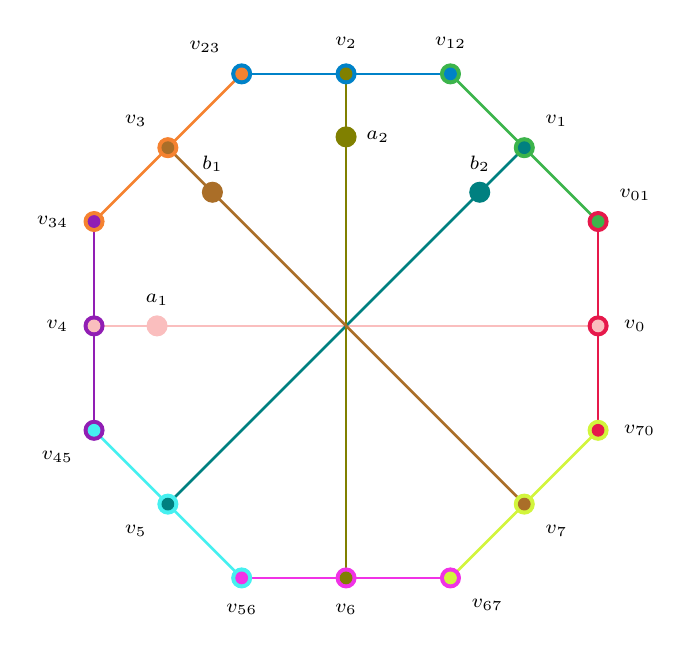
\begin{tikzpicture}[scale=1.6,every label/.style={font=\scriptsize}]
  \def\Rmid{2}
  \def\Rcor{2.1648}% Drawing radius only; unrelated to the algebraic coordinates.
  \def\Rinn{1.5}
  \foreach \i/\j/\ang in {
    0/1/22.5,1/2/67.5,2/3/112.5,3/4/157.5,
    4/5/202.5,5/6/247.5,6/7/292.5,7/0/337.5
  }{\coordinate (v\i\j) at (\ang:\Rcor);}
  \foreach \i/\ang in {
    0/0,1/45,2/90,3/135,4/180,5/225,6/270,7/315
  }{\coordinate (v\i) at (\ang:\Rmid);}
  \coordinate (a1) at (180:\Rinn);
  \coordinate (a2) at (90:\Rinn);
  \coordinate (b1) at (135:\Rinn);
  \coordinate (b2) at (45:\Rinn);

  \draw[ctxline,draw=ctx1] (v70)--(v01);
  \draw[ctxline,draw=ctx2] (v01)--(v12);
  \draw[ctxline,draw=ctx3] (v12)--(v23);
  \draw[ctxline,draw=ctx4] (v23)--(v34);
  \draw[ctxline,draw=ctx5] (v34)--(v45);
  \draw[ctxline,draw=ctx6] (v45)--(v56);
  \draw[ctxline,draw=ctx7] (v56)--(v67);
  \draw[ctxline,draw=ctx8] (v67)--(v70);
  \draw[ctxline,draw=ctx9] (v0)--(v4);
  \draw[ctxline,draw=ctx10] (v1)--(v5);
  \draw[ctxline,draw=ctx11] (v2)--(v6);
  \draw[ctxline,draw=ctx12] (v3)--(v7);

  \twodotlabel{ctx1}{ctx2}{above right}{$v_{01}$}{(v01)}
  \twodotlabel{ctx2}{ctx3}{above}{$v_{12}$}{(v12)}
  \twodotlabel{ctx3}{ctx4}{above left}{$v_{23}$}{(v23)}
  \twodotlabel{ctx4}{ctx5}{left}{$v_{34}$}{(v34)}
  \twodotlabel{ctx5}{ctx6}{below left}{$v_{45}$}{(v45)}
  \twodotlabel{ctx6}{ctx7}{below}{$v_{56}$}{(v56)}
  \twodotlabel{ctx7}{ctx8}{below right}{$v_{67}$}{(v67)}
  \twodotlabel{ctx8}{ctx1}{right}{$v_{70}$}{(v70)}
  \twodotlabel{ctx1}{ctx9}{right}{$v_0$}{(v0)}
  \twodotlabel{ctx2}{ctx10}{above right}{$v_1$}{(v1)}
  \twodotlabel{ctx3}{ctx11}{above}{$v_2$}{(v2)}
  \twodotlabel{ctx4}{ctx12}{above left}{$v_3$}{(v3)}
  \twodotlabel{ctx5}{ctx9}{left}{$v_4$}{(v4)}
  \twodotlabel{ctx6}{ctx10}{below left}{$v_5$}{(v5)}
  \twodotlabel{ctx7}{ctx11}{below}{$v_6$}{(v6)}
  \twodotlabel{ctx8}{ctx12}{below right}{$v_7$}{(v7)}
  \node[circle,fill=ctx9,draw=ctx9,minimum size=7.2pt,inner sep=0pt,
        label={[font=\scriptsize]above:{$a_1$}}] at (a1) {};
  \node[circle,fill=ctx11,draw=ctx11,minimum size=7.2pt,inner sep=0pt,
        label={[font=\scriptsize]right:{$a_2$}}] at (a2) {};
  \node[circle,fill=ctx12,draw=ctx12,minimum size=7.2pt,inner sep=0pt,
        label={[font=\scriptsize]above:{$b_1$}}] at (b1) {};
  \node[circle,fill=ctx10,draw=ctx10,minimum size=7.2pt,inner sep=0pt,
        label={[font=\scriptsize]above:{$b_2$}}] at (b2) {};
\end{tikzpicture}
\caption{The 20-ray hypergraph $\Htwenty$.  The eight perimeter contexts
$E_0,\ldots,E_7$ form the octagon; the four inner contexts join opposite
midpoints through $a_1,a_2,b_1,b_2$.  Each color denotes one context.}
\label{fig:h20}
\end{figure*}

\subsection{The covering identity}

Consider the two collections of six contexts
\begin{align*}
 \mathcal A&=\{D_0,D_2,E_1,E_3,E_5,E_7\},\\
 \mathcal B&=\{D_1,D_3,E_0,E_2,E_4,E_6\}.
\end{align*}
Every midpoint and every corner occurs exactly once in each collection.
Only the two $a$-vertices occur in $\mathcal A$, and only the two
$b$-vertices occur in $\mathcal B$.  Summing Eq.~\eqref{eq:context-sum}
over the two collections and subtracting therefore gives
\begin{equation}
 P_{a_1}+P_{a_2}=P_{b_1}+P_{b_2}.
 \label{eq:covering-identity}
\end{equation}
This identity is combinatorial: it holds in every real or complex
three-dimensional representation of $\Htwenty$.

\subsection{An exact faithful representation over
\texorpdfstring{$\C^3$}{C3}}

Set
\begin{equation}
 \begin{aligned}
 C&=\frac{49-5\sqrt{69}}{26},&s&=\sqrt C,\\
 N&=1+C,&r&=\sqrt N.
 \end{aligned}
 \label{eq:C-definition}
\end{equation}
The number $C$ is the smaller positive root of
\begin{equation}
 13C^2-49C+13=0,
 \label{eq:C-polynomial}
\end{equation}
so $0<C<1$.  Define the unit phases
\begin{align}
 \eta&=\frac{5+12\ii}{13},\label{eq:eta}\\
 \zeta&=\frac{14+6\sqrt{69}}{65}
 +\ii\frac{4\sqrt{69}-21}{65}.
 \label{eq:zeta}
\end{align}
Let
\begin{align*}
 (\mu_0,\ldots,\mu_7)&=(-1,\eta,1,-\eta,-1,\eta,1,-\eta),\\
 (\tau_0,\ldots,\tau_7)&=(1,\zeta,-\ii,-\ii\zeta,
 -1,-\zeta,\ii,\ii\zeta).
\end{align*}
The inner and midpoint rays are represented by
\begin{align}
 a_1&=(s,1,0),&a_2&=(s,-1,0),\nonumber\\
 b_1&=(s,\eta,0),&b_2&=(s,-\eta,0),
 \label{eq:h20-inner-vectors}\\
 v_j&=(1,s\mu_j,r\tau_j),&&j=0,\ldots,7.
 \label{eq:h20-midpoints}
\end{align}
For $j$ modulo eight, define
\begin{equation}
 v_{j,j+1}=v_j\boxtimes v_{j+1}.
 \label{eq:h20-corners}
\end{equation}
Equivalently, Eq.~\eqref{eq:h20-corners} is the explicit formula
\begin{multline}
 v_{j,j+1}=\bigl(
 sr(\bar\mu_j\bar\tau_{j+1}-\bar\tau_j\bar\mu_{j+1}),\\
 r(\bar\tau_j-\bar\tau_{j+1}),
 s(\bar\mu_{j+1}-\bar\mu_j)\bigr).
 \label{eq:h20-corner-formula}
\end{multline}

\begin{theorem}
\label{thm:h20-complex}
Equations~\eqref{eq:C-definition}--\eqref{eq:h20-corner-formula}
give a faithful orthogonal representation of $\Htwenty$ in $\C^3$.
\end{theorem}

\begin{proof}
First, $|\eta|=1$.  Write $\zeta=x+\ii y$.  The four inner contexts
follow directly from $r^2=N$, $|\eta|=|\zeta|=1$, and the antipodal
relations $\mu_{j+4}=\mu_j$, $\tau_{j+4}=-\tau_j$.  For example,
\[
 \langle a_1,v_0\rangle=0,\qquad
 \langle v_0,v_4\rangle=1+C-r^2=0,
\]
and
\[
 \langle b_2,v_1\rangle=0,\qquad
 \langle v_1,v_5\rangle=1+C-r^2|\zeta|^2=0.
\]
The other two inner contexts are identical calculations.

By construction, $v_{j,j+1}$ is orthogonal to $v_j$ and $v_{j+1}$.
It remains to prove orthogonality of the two corner rays in every
perimeter context.  Put
\[
 G_{jk}=\langle v_j,v_k\rangle
 =1+C\bar\mu_j\mu_k+N\bar\tau_j\tau_k.
\]
Lemma~\ref{lem:gram-closure} reduces the eight remaining conditions to
\begin{equation}
 G_{j-1,j}G_{j,j+1}=G_{j-1,j+1}G_{j,j},
 \qquad j=0,\ldots,7.
 \label{eq:h20-closure}
\end{equation}
Substituting the cyclic patterns for $\mu_j$ and $\tau_j$ reduces all eight
conditions to common real and imaginary equations once $x^2+y^2=1$.
Separating those parts gives
\begin{align}
 7Cx-17Cy-13C-13x+13y+13&=0,
 \label{eq:closure-real}
\end{align}
and
\begin{multline}
 -7C^2x+17C^2y+13C^2-20Cx+30Cy\\
 {}+2C-13x+13y+13=0.
 \label{eq:closure-imag}
\end{multline}
Solving these two linear equations for $x$ and $y$ gives
\begin{equation}
 x=\frac{104-76C}{65(1+C)},\qquad
 y=\frac{39-81C}{65(1+C)}.
 \label{eq:xy-C}
\end{equation}
For these values,
\begin{equation}
 x^2+y^2-1=
 \frac{48(13C^2-49C+13)}{325(1+C)^2}=0.
 \label{eq:zeta-unit}
\end{equation}
Using the smaller root in Eq.~\eqref{eq:C-polynomial},
Eq.~\eqref{eq:xy-C} is exactly the phase in Eq.~\eqref{eq:zeta}.
Thus all twelve triples are contexts.

It remains to exclude unintended orthogonalities and ray coincidences.
The exact overlap certificate in Appendix~\ref{app:faithfulness} shows
that the 36 prescribed unordered pairs have zero overlap, whereas the
154 unprescribed pairs have squared normalized overlaps between $1/25$
and $4/5$.  Hence every unprescribed inner product is nonzero and no two
displayed vectors are proportional.  The representation is faithful.
\end{proof}

The two inner pairs indeed decompose the same operator.  Since all four
vectors have squared norm $N$ and $|\eta|=1$,
\begin{equation}
 P_{a_1}+P_{a_2}=P_{b_1}+P_{b_2}
 =\frac{2}{N}\operatorname{diag}(C,1,0).
 \label{eq:complex-two-sum}
\end{equation}
Their within-pair inner products are $C-1\ne0$, and the four rays are
distinct because $\eta\notin\{1,-1\}$.

\subsection{Nonexistence over \texorpdfstring{$\R^3$}{R3}}

\begin{theorem}
\label{thm:h20-real}
The hypergraph $\Htwenty$ has no faithful orthogonal representation in
$\R^3$.
\end{theorem}

\begin{proof}
Suppose a faithful real representation existed.  The covering argument
is independent of the field, so Eq.~\eqref{eq:covering-identity} would
hold.  Faithfulness implies that $a_1,a_2$ are distinct and
nonorthogonal, because they do not share a context; the same is true of
$b_1,b_2$.  Lemma~\ref{lem:real-rigidity} then identifies the unordered
pair of $b$-rays with the unordered pair of $a$-rays.  This contradicts
the requirement that four distinct vertices label four distinct rays.
\end{proof}

\section{The 21-ray orthogonal augmentation}
\label{sec:h21}

Add one vertex $c$ and two contexts
\begin{equation}
 F_a=\{a_1,c,a_2\},\qquad F_b=\{b_1,c,b_2\}
 \label{eq:added-contexts}
\end{equation}
to $\Htwenty$.  The result is the 21-vertex, 14-context hypergraph
$\Htwentyone$ shown in Fig.~\ref{fig:h21}.  The added contexts force both
inner pairs to be orthogonal and to have the same one-dimensional
orthogonal complement.

\begin{figure*}[t]
\centering
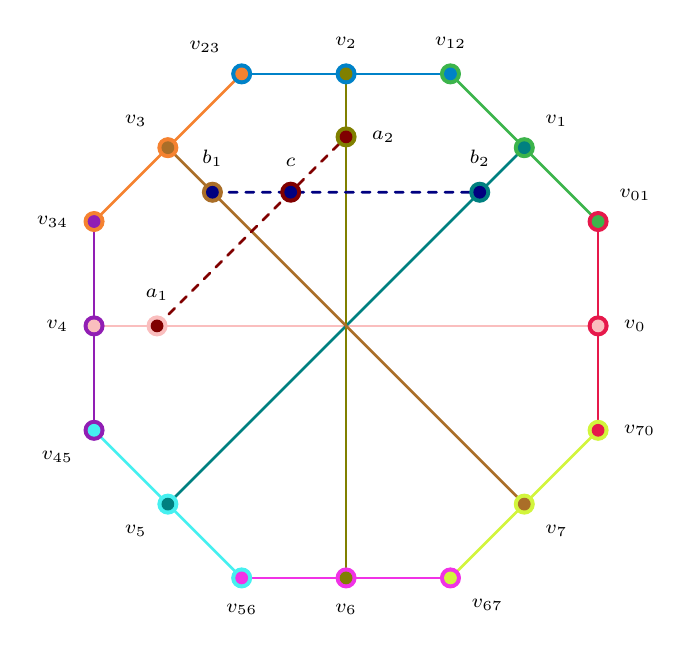
\begin{tikzpicture}[scale=1.6,every label/.style={font=\scriptsize}]
  \def\Rmid{2}
  \def\Rcor{2.1648}% Drawing radius only; unrelated to the algebraic coordinates.
  \def\Rinn{1.5}
  \foreach \i/\j/\ang in {
    0/1/22.5,1/2/67.5,2/3/112.5,3/4/157.5,
    4/5/202.5,5/6/247.5,6/7/292.5,7/0/337.5
  }{\coordinate (v\i\j) at (\ang:\Rcor);}
  \foreach \i/\ang in {
    0/0,1/45,2/90,3/135,4/180,5/225,6/270,7/315
  }{\coordinate (v\i) at (\ang:\Rmid);}
  \coordinate (a1) at (180:\Rinn);
  \coordinate (a2) at (90:\Rinn);
  \coordinate (b1) at (135:\Rinn);
  \coordinate (b2) at (45:\Rinn);
  \coordinate (c) at ($(a1)!0.70710678!(a2)$);

  \draw[ctxline,draw=ctx1] (v70)--(v01);
  \draw[ctxline,draw=ctx2] (v01)--(v12);
  \draw[ctxline,draw=ctx3] (v12)--(v23);
  \draw[ctxline,draw=ctx4] (v23)--(v34);
  \draw[ctxline,draw=ctx5] (v34)--(v45);
  \draw[ctxline,draw=ctx6] (v45)--(v56);
  \draw[ctxline,draw=ctx7] (v56)--(v67);
  \draw[ctxline,draw=ctx8] (v67)--(v70);
  \draw[ctxline,draw=ctx9] (v0)--(v4);
  \draw[ctxline,draw=ctx10] (v1)--(v5);
  \draw[ctxline,draw=ctx11] (v2)--(v6);
  \draw[ctxline,draw=ctx12] (v3)--(v7);
  \draw[ctxline,dashed,draw=ctx13] (a1)--(c)--(a2);
  \draw[ctxline,dashed,draw=ctx14] (b1)--(c)--(b2);

  \twodotlabel{ctx1}{ctx2}{above right}{$v_{01}$}{(v01)}
  \twodotlabel{ctx2}{ctx3}{above}{$v_{12}$}{(v12)}
  \twodotlabel{ctx3}{ctx4}{above left}{$v_{23}$}{(v23)}
  \twodotlabel{ctx4}{ctx5}{left}{$v_{34}$}{(v34)}
  \twodotlabel{ctx5}{ctx6}{below left}{$v_{45}$}{(v45)}
  \twodotlabel{ctx6}{ctx7}{below}{$v_{56}$}{(v56)}
  \twodotlabel{ctx7}{ctx8}{below right}{$v_{67}$}{(v67)}
  \twodotlabel{ctx8}{ctx1}{right}{$v_{70}$}{(v70)}
  \twodotlabel{ctx1}{ctx9}{right}{$v_0$}{(v0)}
  \twodotlabel{ctx2}{ctx10}{above right}{$v_1$}{(v1)}
  \twodotlabel{ctx3}{ctx11}{above}{$v_2$}{(v2)}
  \twodotlabel{ctx4}{ctx12}{above left}{$v_3$}{(v3)}
  \twodotlabel{ctx5}{ctx9}{left}{$v_4$}{(v4)}
  \twodotlabel{ctx6}{ctx10}{below left}{$v_5$}{(v5)}
  \twodotlabel{ctx7}{ctx11}{below}{$v_6$}{(v6)}
  \twodotlabel{ctx8}{ctx12}{below right}{$v_7$}{(v7)}
  \twodotlabel{ctx9}{ctx13}{above}{$a_1$}{(a1)}
  \twodotlabel{ctx11}{ctx13}{right}{$a_2$}{(a2)}
  \twodotlabel{ctx12}{ctx14}{above}{$b_1$}{(b1)}
  \twodotlabel{ctx10}{ctx14}{above}{$b_2$}{(b2)}
  \twodotlabel{ctx13}{ctx14}{above}{$c$}{(c)}
\end{tikzpicture}
\caption{The 21-ray hypergraph $\Htwentyone$.  The twelve solid contexts
are those of $\Htwenty$; the two dashed contexts meet at the new vertex
$c$.}
\label{fig:h21}
\end{figure*}

\subsection{Exact coordinates over \texorpdfstring{$\C^3$}{C3}}

Let
\begin{equation}
 p=\frac{\sqrt{14}+\sqrt2}{4},\qquad
 q=\frac{\sqrt{14}-\sqrt2}{4}.
 \label{eq:pq}
\end{equation}
Then
\begin{equation}
 p^2+q^2=2,\qquad pq=\frac34.
 \label{eq:pq-identities}
\end{equation}
Choose
\begin{align}
 c&=(0,0,1),\nonumber\\
 a_1&=(1,1,0),&a_2&=(1,-1,0),\nonumber\\
 b_1&=(1,\ii,0),&b_2&=(1,-\ii,0),
 \label{eq:h21-inner}
\end{align}
and the eight midpoint representatives
\begin{align}
 v_0&=(1,-1,\sqrt2),&v_4&=(1,-1,-\sqrt2),\nonumber\\
 v_1&=(1,\ii,p+\ii q),&v_5&=(1,\ii,-p-\ii q),\nonumber\\
 v_2&=(1,1,-\ii\sqrt2),&v_6&=(1,1,\ii\sqrt2),\nonumber\\
 v_3&=(1,-\ii,q-\ii p),&v_7&=(1,-\ii,-q+\ii p).
 \label{eq:h21-midpoints}
\end{align}
The eight corner representatives are
\begin{align}
 v_{01}&=(-p+\ii(q+\sqrt2),\ \sqrt2-p+\ii q,\ 1-\ii),\nonumber\\
 v_{12}&=(\sqrt2-p+\ii q,\ p-\ii(q+\sqrt2),\ 1+\ii),\nonumber\\
 v_{23}&=(q+\sqrt2+\ii p,\ -q+\ii(\sqrt2-p),\ -1+\ii),\nonumber\\
 v_{34}&=(q+\ii(p-\sqrt2),\ q+\sqrt2+\ii p,\ -1-\ii),\nonumber\\
 v_{45}&=(p-\ii(q+\sqrt2),\ -\sqrt2+p-\ii q,\ 1-\ii),\nonumber\\
 v_{56}&=(-\sqrt2+p-\ii q,\ -p+\ii(q+\sqrt2),\ 1+\ii),\nonumber\\
 v_{67}&=(-q-\sqrt2-\ii p,\ q-\ii(\sqrt2-p),\ -1+\ii),\nonumber\\
 v_{70}&=(-q-\ii(p-\sqrt2),\ -q-\sqrt2-\ii p,\ -1-\ii).
 \label{eq:h21-corners}
\end{align}

\begin{theorem}
\label{thm:h21-complex}
Equations~\eqref{eq:pq}--\eqref{eq:h21-corners} give a faithful
orthogonal representation of $\Htwentyone$ in $\C^3$.
\end{theorem}

\begin{proof}
The two added contexts are immediate from Eq.~\eqref{eq:h21-inner}.
For the original inner contexts, representative calculations are
\begin{align*}
 \langle a_1,v_0\rangle&=0,&
 \langle v_0,v_4\rangle&=1+1-2=0,\\
 \langle b_2,v_1\rangle&=0,&
 \langle v_1,v_5\rangle&=2-(p^2+q^2)=0.
\end{align*}
The two remaining inner contexts follow in the same way.

Direct evaluation of the Hermitian cross product gives, exactly,
\[
 v_{j,j+1}=v_j\boxtimes v_{j+1}
\]
for each representative in Eq.~\eqref{eq:h21-corners}.  Hence every
corner is orthogonal to its two incident midpoints.  Substitution in the
Gram closure identity~\eqref{eq:gram-closure} reduces the eight remaining
perimeter inner products to the two relations in
Eq.~\eqref{eq:pq-identities}; they therefore vanish.

Finally, Appendix~\ref{app:faithfulness} gives an exact check of all 210
unordered pairs.  The 42 pairs prescribed by the fourteen contexts have
zero overlap.  Every remaining pair has squared normalized overlap
either $1/4$ or $1/2$.  Thus there are no additional orthogonalities and
no ray coincidences.
\end{proof}

\subsection{Nonexistence over \texorpdfstring{$\R^3$}{R3}}

\begin{theorem}
\label{thm:h21-real}
The hypergraph $\Htwentyone$ has no faithful orthogonal representation
in $\R^3$.
\end{theorem}

\begin{proof}
Assume that a faithful real representation exists.  A global orthogonal
transformation and independent rescalings of ray representatives allow
us to set
\begin{equation}
 c=(0,0,1),\qquad a_1=(1,0,0),\qquad a_2=(0,1,0).
 \label{eq:real-normal-a}
\end{equation}
The second added context lies in the plane $c^\perp$, so for some angle
$\theta$,
\begin{equation}
 b_1=(\cos\theta,\sin\theta,0),\qquad
 b_2=(-\sin\theta,\cos\theta,0).
 \label{eq:real-normal-b}
\end{equation}
Faithfulness excludes $\theta\in\frac{\pi}{2}\mathbb Z$, since those
values identify a $b$-ray with an $a$-ray.  Put
\begin{equation}
 m=\tan\theta\ne0,\qquad M=1+m^2.
 \label{eq:mM}
\end{equation}

Write a representative vector of a midpoint ray as
$v_j=(X_j,Y_j,Z_j)$.  No midpoint ray can lie in $c^\perp$.
Indeed, a planar vector orthogonal to the inner ray in its
context is proportional to the other member of one of the two planar
bases $\{a_1,a_2\}$ or $\{b_1,b_2\}$, contradicting faithfulness.
Thus $Z_j\ne0$ for every $j$, and each representative may be rescaled to
\begin{equation}
 v_j=(X_j,Y_j,1).
 \label{eq:affine-midpoints}
\end{equation}

The inner contexts $D_0,D_1,D_3$ imply
\begin{align}
 X_0&=X_4=0,&Y_0Y_4+1&=0,
 \label{eq:D0-real}\\
 Y_1&=mX_1,&Y_5&=mX_5,&MX_1X_5+1&=0,
 \label{eq:D1-real}\\
 X_3&=-mY_3,&X_7&=-mY_7,&MY_3Y_7+1&=0.
 \label{eq:D3-real}
\end{align}
In particular,
\begin{equation}
 X_5=-\frac1{MX_1},\qquad
 Y_7=-\frac1{MY_3},
 \label{eq:X5Y7}
\end{equation}
and $X_1Y_3\ne0$.

The corner rays can be eliminated from the perimeter by the real form
of Lemma~\ref{lem:gram-closure}.  At $j=0$,
Eq.~\eqref{eq:gram-closure} factors as
\begin{equation}
 Y_0\bigl((mX_1Y_7-1)Y_0+Y_7+mX_1\bigr)=0.
 \label{eq:j0-factor}
\end{equation}
The first factor cannot vanish because of Eq.~\eqref{eq:D0-real}.
Moreover, the coefficient $1-mX_1Y_7$ cannot vanish: otherwise
Eq.~\eqref{eq:j0-factor} would also give $Y_7+mX_1=0$, and the two
relations would imply $-m^2X_1^2=1$.  Therefore
\begin{equation}
 Y_0=\frac{Y_7+mX_1}{1-mX_1Y_7}.
 \label{eq:Y0-first}
\end{equation}
The closure equation at $j=4$ gives analogously
\begin{equation}
 Y_4=\frac{Y_3+mX_5}{1-mY_3X_5},
 \label{eq:Y4-first}
\end{equation}
with a nonzero denominator.

Substituting Eq.~\eqref{eq:X5Y7} into
Eqs.~\eqref{eq:Y0-first} and~\eqref{eq:Y4-first} yields
\begin{equation}
 Y_0=\frac{mMX_1Y_3-1}{MY_3+mX_1},\qquad
 Y_4=\frac{MX_1Y_3-m}{MX_1+mY_3}.
 \label{eq:Y0Y4-final}
\end{equation}
Set $u=X_1Y_3$.  The remaining equation $Y_0Y_4=-1$ becomes
\begin{equation}
 (mMu-1)(Mu-m)=-(mX_1+MY_3)(MX_1+mY_3).
 \label{eq:cross-multiplied}
\end{equation}
Expanding the left-hand side gives
\begin{align*}
 (mMu-1)(Mu-m)
 &=mM^2u^2-M(m^2+1)u+m\\
 &=mM^2u^2-M^2u+m,
\end{align*}
where the second equality uses $M=1+m^2$.
The right-hand side is
\[
 -u(M^2+m^2)-mM(X_1^2+Y_3^2).
\]
After cancellation and division by $m\ne0$, Eq.~\eqref{eq:cross-multiplied}
is therefore equivalent to the master equation
\begin{equation}
 M^2u^2+mu+1+M(X_1^2+Y_3^2)=0.
 \label{eq:master}
\end{equation}

Since $X_1,Y_3$ are real,
$X_1^2+Y_3^2\ge2|X_1Y_3|=2|u|$.  The left-hand side of
Eq.~\eqref{eq:master} is consequently at least
\begin{align*}
 M^2u^2+mu+1+2M|u|
 &\ge 1+M^2u^2+|u|(2M-|m|)\\
 &\ge1.
\end{align*}
Here, with $t=|m|$,
\[
 2M-|m|=2t^2-t+2=2\left(t-\frac14\right)^2+\frac{15}{8}>0.
\]
This contradicts
Eq.~\eqref{eq:master}, and the assumed real representation cannot exist.
\end{proof}

\section{A finite transition-probability field witness}
\label{sec:operational}

We now turn the two exact representability separations into a calibrated
prepare-and-test task.  For $n\in\{20,21\}$, let $V_n$ be the vertex set of
$\mathsf H_n$, let $\psi_v^{(n)}\in\C^3$ be the complex representative
displayed above, and define the ideal transition table
\begin{equation}
 T_{uv}^{(n)}=Q\bigl(\psi_u^{(n)},\psi_v^{(n)}\bigr),
 \qquad u,v\in V_n.
 \label{eq:target-table}
\end{equation}
Operationally, label $v$ specifies both the preparation
$\rho_v=P_{\psi_v^{(n)}}$ and the reciprocal yes--no test
$E_v=P_{\psi_v^{(n)}}$.  The ideal accepting probability is then
$p(v|u)=\operatorname{Tr}(\rho_uE_v)=T_{uv}^{(n)}$.

To compare with real qutrits, fix any ordering of $V_n$ and define the
uniform real fitting error
\begin{equation}
 \varepsilon_{\R}^{(n)}=
 \min_{\substack{r_v\in\R^3,\ \|r_v\|=1\\v\in V_n}}
 \ \max_{u<v}
 \left| (r_u^{\mathsf T}r_v)^2-T_{uv}^{(n)}\right|.
 \label{eq:real-gap}
\end{equation}
This comparison is dimension bounded and calibrated: each test is assumed to
be the rank-one projector associated with the correspondingly labeled pure
preparation.  It is not a device-independent Bell or contextuality scenario.

\begin{theorem}[Positive real-qutrit gap]
\label{thm:operational-gap}
The ideal tables $T^{(20)}$ and $T^{(21)}$ are realized exactly by complex
qutrits, whereas
\begin{equation}
 \varepsilon_{\R}^{(20)}>0,
 \qquad
 \varepsilon_{\R}^{(21)}>0.
 \label{eq:positive-gaps}
\end{equation}
For $\Htwentyone$, every off-diagonal target probability belongs to
$\{0,1/4,1/2\}$.
\end{theorem}

\begin{proof}
The displayed complex representatives realize Eq.~\eqref{eq:target-table}, so
the corresponding complex fitting error is zero.  For the real problem, the
domain $(S^2)^{|V_n|}$ in Eq.~\eqref{eq:real-gap} is compact and the objective
is continuous; hence the minimum is attained.

Suppose that this minimum were zero.  Then some family of real unit vectors
would reproduce every target entry exactly.  The target value is zero for
precisely the pairs prescribed by the contexts and is strictly positive for
every other pair.  Moreover, for distinct vertices the target is strictly
less than one: Appendix~\ref{app:faithfulness} gives the bound $T_{uv}^{(20)}
\le4/5$ and gives $T_{uv}^{(21)}\in\{1/4,1/2\}$ for every nonorthogonal pair.
The real vectors would therefore have exactly the prescribed
orthogonalities, no ray coincidences, and no unintended orthogonalities.
They would constitute a faithful orthogonal representation of
$\mathsf H_n$ in $\R^3$, contradicting Theorem~\ref{thm:h20-real} for $n=20$
and Theorem~\ref{thm:h21-real} for $n=21$.  Thus both real minima are strictly
positive.  The final statement follows from the exact overlap inventory in
Appendix~\ref{app:faithfulness}.
\end{proof}

Theorem~\ref{thm:operational-gap} supplies a finite robustness statement:
every reciprocal real-qutrit model differs from the ideal table in at least
one tested transition by at least $\varepsilon_{\R}^{(n)}$.  Consequently, a
calibrated experiment whose systematic and statistical uncertainty places
the complete table within a smaller uniform error rules out that model class.
The proof establishes a nonzero gap but does not determine its optimal value.
Computing a certified lower bound, optimizing the weights in an averaged
score, and finding the smallest subset of transitions that retains a gap are
natural next steps toward an economical implementation.  The
$\Htwentyone$ table is especially attractive for this purpose because its
210 unordered off-diagonal transition pairs have only three ideal probability
values.

\section{Faithful realification in six dimensions}
\label{sec:realification}

Theorems~\ref{thm:h20-real} and~\ref{thm:h21-real} keep the ambient
dimension fixed.  When dimension doubling is allowed, both hypergraphs have
faithful real representations.  We first recall the finite construction and
then give explicit phase choices for the present
coordinates~\cite{svozil-2025-rvc}.

\begin{theorem}[Phase-adjusted realification]
\label{thm:realification}
Every finite faithful orthogonal representation by rays in $\C^3$ induces a
faithful orthogonal representation of the same hypergraph by rays in $\R^6$.
\end{theorem}

\begin{proof}
Let $\psi_1,\ldots,\psi_N\in\C^3$ be nonzero representatives and put
$c_{k\ell}=\langle\psi_k,\psi_\ell\rangle$.  Define the canonical
realification
\begin{equation}
 \Phi_0(z_1,z_2,z_3)
 = (\Re z_1,\Re z_2,\Re z_3,\Im z_1,\Im z_2,\Im z_3).
 \label{eq:canonical-realification}
\end{equation}
For phases $\theta_k\in\R$, set
$R_k=\Phi_0(e^{\ii\theta_k}\psi_k)$.  Direct expansion gives
\begin{equation}
 R_k\mathbin{\cdot}R_\ell
 =\Re\!\left(e^{\ii(\theta_\ell-\theta_k)}c_{k\ell}\right).
 \label{eq:realified-dot}
\end{equation}
Thus $c_{k\ell}=0$ implies $R_k\cdot R_\ell=0$ for every phase choice.
If $c_{k\ell}\ne0$, write
$c_{k\ell}=|c_{k\ell}|e^{\ii\varphi_{k\ell}}$.  The right-hand side of
Eq.~\eqref{eq:realified-dot} vanishes precisely when
\begin{equation}
 \theta_\ell-\theta_k+\varphi_{k\ell}
 \equiv\frac{\pi}{2}\pmod\pi.
 \label{eq:forbidden-phase}
\end{equation}

Choose $\theta_1,\ldots,\theta_N$ inductively.  Suppose that the first $m-1$
phases have been fixed.  For each $k<m$ with $c_{km}\ne0$, the unwanted
orthogonality equation $R_k\mathbin{\cdot}R_m=0$ excludes, by
Eq.~\eqref{eq:forbidden-phase}, exactly two values of $\theta_m$ modulo
$2\pi$.  Their union is finite, so a phase outside it exists.  Continuing
through $m=N$ makes the real dot product nonzero for every originally
nonorthogonal pair, while all original orthogonalities remain zero.

It remains only to check ray distinctness.  If $R_k$ and $R_\ell$ were real
proportional, then $e^{\ii\theta_k}\psi_k$ and
$e^{\ii\theta_\ell}\psi_\ell$ would be real proportional and hence would
represent the same complex ray.  Faithfulness of the original representation
excludes this.  Therefore the realified representation is faithful.
\end{proof}

For explicit coordinates it is convenient to parametrize the phase by a real
number $t$:
\begin{equation}
 \lambda_t=\frac{1+\ii t}{\sqrt{1+t^2}},\qquad
 \Phi_t(z)=\Phi_0(\lambda_tz).
 \label{eq:lambda-t}
\end{equation}
Writing $z=x+\ii y$ with $x,y\in\R^3$ gives the entirely real formula
\begin{equation}
 \Phi_t(x+\ii y)=\frac{(x-ty,\ y+tx)}{\sqrt{1+t^2}}\in\R^6.
 \label{eq:explicit-realification}
\end{equation}
Moreover,
\begin{equation}
 \Phi_{t_u}(u)\mathbin{\cdot}\Phi_{t_v}(v)
 =\Re\!\left(
 \frac{(1-\ii t_u)(1+\ii t_v)}
 {\sqrt{(1+t_u^2)(1+t_v^2)}}\langle u,v\rangle
 \right).
 \label{eq:t-dot}
\end{equation}

\begin{corollary}[Explicit real six-dimensional coordinates]
\label{cor:r6}
Let $\psi_v^{(20)}$ denote the representatives in
Eqs.~\eqref{eq:C-definition}--\eqref{eq:h20-corner-formula}.  Define
\begin{equation}
 t_v^{(20)}=
 \begin{cases}
  1,&v\in\{v_{34},v_{45},v_{56}\},\\
  2,&v\in\{v_{67},v_{70}\},\\
  0,&\text{otherwise}.
 \end{cases}
 \label{eq:t20}
\end{equation}
Then $R_v^{(20)}=\Phi_{t_v^{(20)}}(\psi_v^{(20)})$ is a faithful orthogonal
representation of $\Htwenty$ in $\R^6$.

Likewise, let $\psi_v^{(21)}$ denote the representatives in
Eqs.~\eqref{eq:pq}--\eqref{eq:h21-corners}, and define
\begin{equation}
 t_v^{(21)}=
 \begin{cases}
  1,&v=v_{45},\\
  2,&v\in\{v_2,v_3,v_6,v_7,v_{34},v_{56},v_{70}\},\\
  3,&v=v_{67},\\
  0,&\text{otherwise}.
 \end{cases}
 \label{eq:t21}
\end{equation}
Then $R_v^{(21)}=\Phi_{t_v^{(21)}}(\psi_v^{(21)})$ is a faithful orthogonal
representation of $\Htwentyone$ in $\R^6$.
\end{corollary}

\begin{proof}
Equations~\eqref{eq:explicit-realification}, \eqref{eq:t20}, and
\eqref{eq:t21} give all six real coordinates directly from the complex
vectors already displayed.  Exact substitution in Eq.~\eqref{eq:t-dot}
gives zero for exactly 36 of the $\binom{20}{2}=190$ pairs in $\Htwenty$,
namely the pairs prescribed by its twelve contexts.  The other 154 real dot
products are nonzero.  For $\Htwentyone$, exactly 42 of the
$\binom{21}{2}=210$ real dot products vanish, namely the pairs prescribed by
its fourteen contexts, and the other 168 are nonzero.  These calculations
take place in the algebraic fields generated by the radicals in the complex
coordinates and by $\sqrt{1+t^2}$; no numerical tolerance is involved.
Ray distinctness follows from Theorem~\ref{thm:realification}.
\end{proof}

Each displayed three-ray context is therefore an orthogonal triple in
$\R^6$, but it spans only a three-dimensional subspace.  Its projector sum
is the rank-three projector onto that subspace, not $I_6$.  This loss of
maximality is precisely why the real six-dimensional representations do not
contradict the two real three-dimensional no-go theorems.

\section{Discussion}

The two no-go proofs expose different field-dependent mechanisms.  For
$\Htwenty$, the context covering forces a rank-two positive operator to have
two disjoint, nonorthogonal decompositions into rank-one projectors.  Complex
relative phases make this possible.  Over the reals, the two simple
eigenvalues determine the two rays, producing the rigidity of
Lemma~\ref{lem:real-rigidity}.  For $\Htwentyone$, the inner pairs are
orthogonal and their common projector sum is the identity on $c^\perp$.
The spectral argument is therefore unavailable.  Compatibility with the
octagonal perimeter instead produces the positive master expression in
Eq.~\eqref{eq:master}.  The second witness is not merely the orthogonal limit
of the first proof; it requires a genuinely different obstruction.

The transition-probability formulation makes explicit what must be observed
in addition to the contexts.  Orthogonality supplies the zero probabilities,
while probabilities strictly between zero and one on every unprescribed pair
exclude both unintended orthogonalities and ray coincidences.  In this
calibrated setting,
faithfulness is therefore not an unmeasured graph-theoretic convention: it is
encoded by the complete table.  For $\Htwentyone$ the ideal experiment is
particularly discrete, because every off-diagonal probability is $0$, $1/4$,
or $1/2$.

The compactness argument in Theorem~\ref{thm:operational-gap} shows that the
field separation survives a finite uniform perturbation.  This conclusion is
qualitative until a certified value of $\varepsilon_{\R}^{(n)}$ is obtained.
The present witness is also not device independent: it assumes pure
three-dimensional preparations, reciprocal rank-one projective tests, and a
calibration identifying equally labeled preparations and tests.  These
assumptions distinguish the result from Bell tests of real versus complex
quantum theory and from KS noncontextuality inequalities.  They also make its
scope precise: the result is a finite field witness for qutrit geometry, not a
falsification of all real-Hilbert-space formulations.

Corollary~\ref{cor:r6} faithfully realizes the same orthogonality pattern in
$\R^6$, where the triples are not complete measurements.  The context sum is
then a rank-three subspace projector, so neither the covering identity nor the
three-dimensional cross-product closure follows.  This removes the underlying
hypergraph obstruction, but the rank-one real rays need not reproduce the
nonzero table entries, and $\R^4$ and $\R^5$ remain unaddressed.

Faithfulness and the full incidence structure are essential: allowing extra
orthogonalities or ray coincidences permits degeneracy, while deleting
contexts weakens the projector identity or closure system.  Thus the complete
labeled vertex--context structure matters.

The next operational questions are quantitative.  Polynomial optimization or
semidefinite relaxations could provide certified lower bounds on
$\varepsilon_{\R}^{(20)}$ and $\varepsilon_{\R}^{(21)}$.  Optimizing a weighted
average score may yield better statistical performance than the uniform norm
in Eq.~\eqref{eq:real-gap}.  It is also natural to search for a smaller subset
of transitions that retains a real-complex gap, and ultimately for a
self-testing or device-independent task generated by the same incidence
mechanisms.

\section{Conclusion}

The configurations $\Htwenty$ and $\Htwentyone$ define two exact finite
transition-probability tables attained by complex qutrits and by no reciprocal
real-qutrit prepare-and-test model.  Their no-go proofs arise from two
different mechanisms: rigidity of a two-projector decomposition and cyclic
closure at the orthogonal limit.  Exact pairwise certificates establish the
complete tables without numerical or coloring assumptions; for
$\Htwentyone$ the off-diagonal probabilities are only $0$, $1/4$, and $1/2$.
Compactness then promotes exact nonrepresentability to a strictly positive
real-qutrit approximation gap.  The $\R^6$ rank-one realifications remove only
the underlying orthogonality obstruction; they neither reproduce the complete
tables nor determine the minimum real dimension.  A certified numerical gap
and a reduced transition set remain steps toward an efficient implementation.

\appendix

\section{Exact faithfulness certificates}
\label{app:faithfulness}

Recall the squared normalized overlap $Q$ from Eq.~\eqref{eq:Q}.  All
calculations below are exact reductions in the
algebraic fields generated by the displayed radicals and phases.  The
reductions and pair counts were independently cross-checked by exact symbolic
arithmetic; no floating-point tolerance is used.

For $\Htwenty$, the 12 contexts prescribe 36 distinct unordered
orthogonal pairs.  Substitution of
Eqs.~\eqref{eq:C-definition}--\eqref{eq:h20-corner-formula}, followed by
reduction with Eq.~\eqref{eq:C-polynomial}, gives $Q=0$ for precisely
those 36 pairs.  For the other 154 pairs, the complete list of values
and multiplicities is:
\begin{equation}
\begin{array}{c@{\;}r@{\quad}c@{\;}r@{\quad}c@{\;}r}
 Q&\text{mult.}&Q&\text{mult.}&Q&\text{mult.}\\ \hline
 \frac1{25}&2&\frac3{10}&8&\frac8{15}&8\\
 \frac3{50}&4&\frac{23}{75}&2&\frac{14}{25}&8\\
 \frac7{75}&8&\frac{49}{150}&8&\frac{16}{25}&2\\
 \frac8{75}&8&\frac{26}{75}&8&\frac7{10}&8\\
 \frac7{50}&8&\frac{28}{75}&8&\frac{59}{75}&2\\
 \frac4{25}&8&\frac{32}{75}&4&\frac45&16\\
 \frac15&16&\frac7{15}&8&&\\[-2pt]
 \frac6{25}&8&\frac{13}{25}&2&&
\end{array}
\label{eq:H20-Q-table}
\end{equation}
The multiplicities sum to 154.  In particular,
\begin{equation}
 \frac1{25}\le Q(x,y)\le\frac45
 \label{eq:H20-Q-bounds}
\end{equation}
for every unprescribed pair.  This proves simultaneously that no such
pair is orthogonal and that no two vertices label the same ray.

For $\Htwentyone$, the 14 contexts prescribe 42 distinct unordered
orthogonal pairs.  Exact substitution of
Eqs.~\eqref{eq:pq-identities}--\eqref{eq:h21-corners} gives zero for
precisely those pairs.  The other 168 pairs split as
\begin{equation}
 \begin{array}{c|cc}
 Q&\frac14&\frac12\\ \hline
 \text{multiplicity}&84&84
 \end{array}.
 \label{eq:H21-Q-table}
\end{equation}
Again every unprescribed overlap lies strictly between zero and one.
This completes the exact faithfulness verification used in
Theorems~\ref{thm:h20-complex} and~\ref{thm:h21-complex}.

\section*{Data availability}

No external data were used.  The hypergraphs, exact coordinates, and complete
pairwise overlap inventories needed to reproduce the reported results are
contained in this article.

\begin{acknowledgments}
During manuscript preparation, the authors used OpenAI Codex (GPT-5) to assist with literature organization, LaTeX editing, exact symbolic checks, and figure/PDF verification; all AI-assisted output was directed and critically reviewed by the authors, who independently verified the mathematics and take full responsibility for the final content, and no AI tool is an author.
This research was funded in part by the Austrian
Science Fund (FWF), Grant DOI \href{https://doi.org/10.55776/PIN5424624}{10.55776/PIN5424624}, and the Czech Science
Foundation (GA\v{C}R), Grant No.~25-20013L.  The authors declare no
conflict of interest.
\end{acknowledgments}

\bibliography{svozil.bib}

\end{document}
